\documentclass{deltares_manual_dfastbe}

\usepackage{tikz}
\usepackage[pipeTables=true]{markdown}

%------------------------------------------------------------------------------
\newcommand{\dfastbe}{\textrm{D-FAST~Bank Erosion}\xspace}
\newcommand{\dflowfm}{\textrm{D-Flow~FM}\xspace}

\hypersetup
{
    pdfauthor   = {Deltares},
    pdftitle    = {\dfastbe},
    pdfkeywords = {Technical Reference \dfastbe}
}

%------------------------------------------------------------------------------
%

%\makeindex

%------------------------------------------------------------------------------
%
\begin{document}
%\pagestyle{empty}
%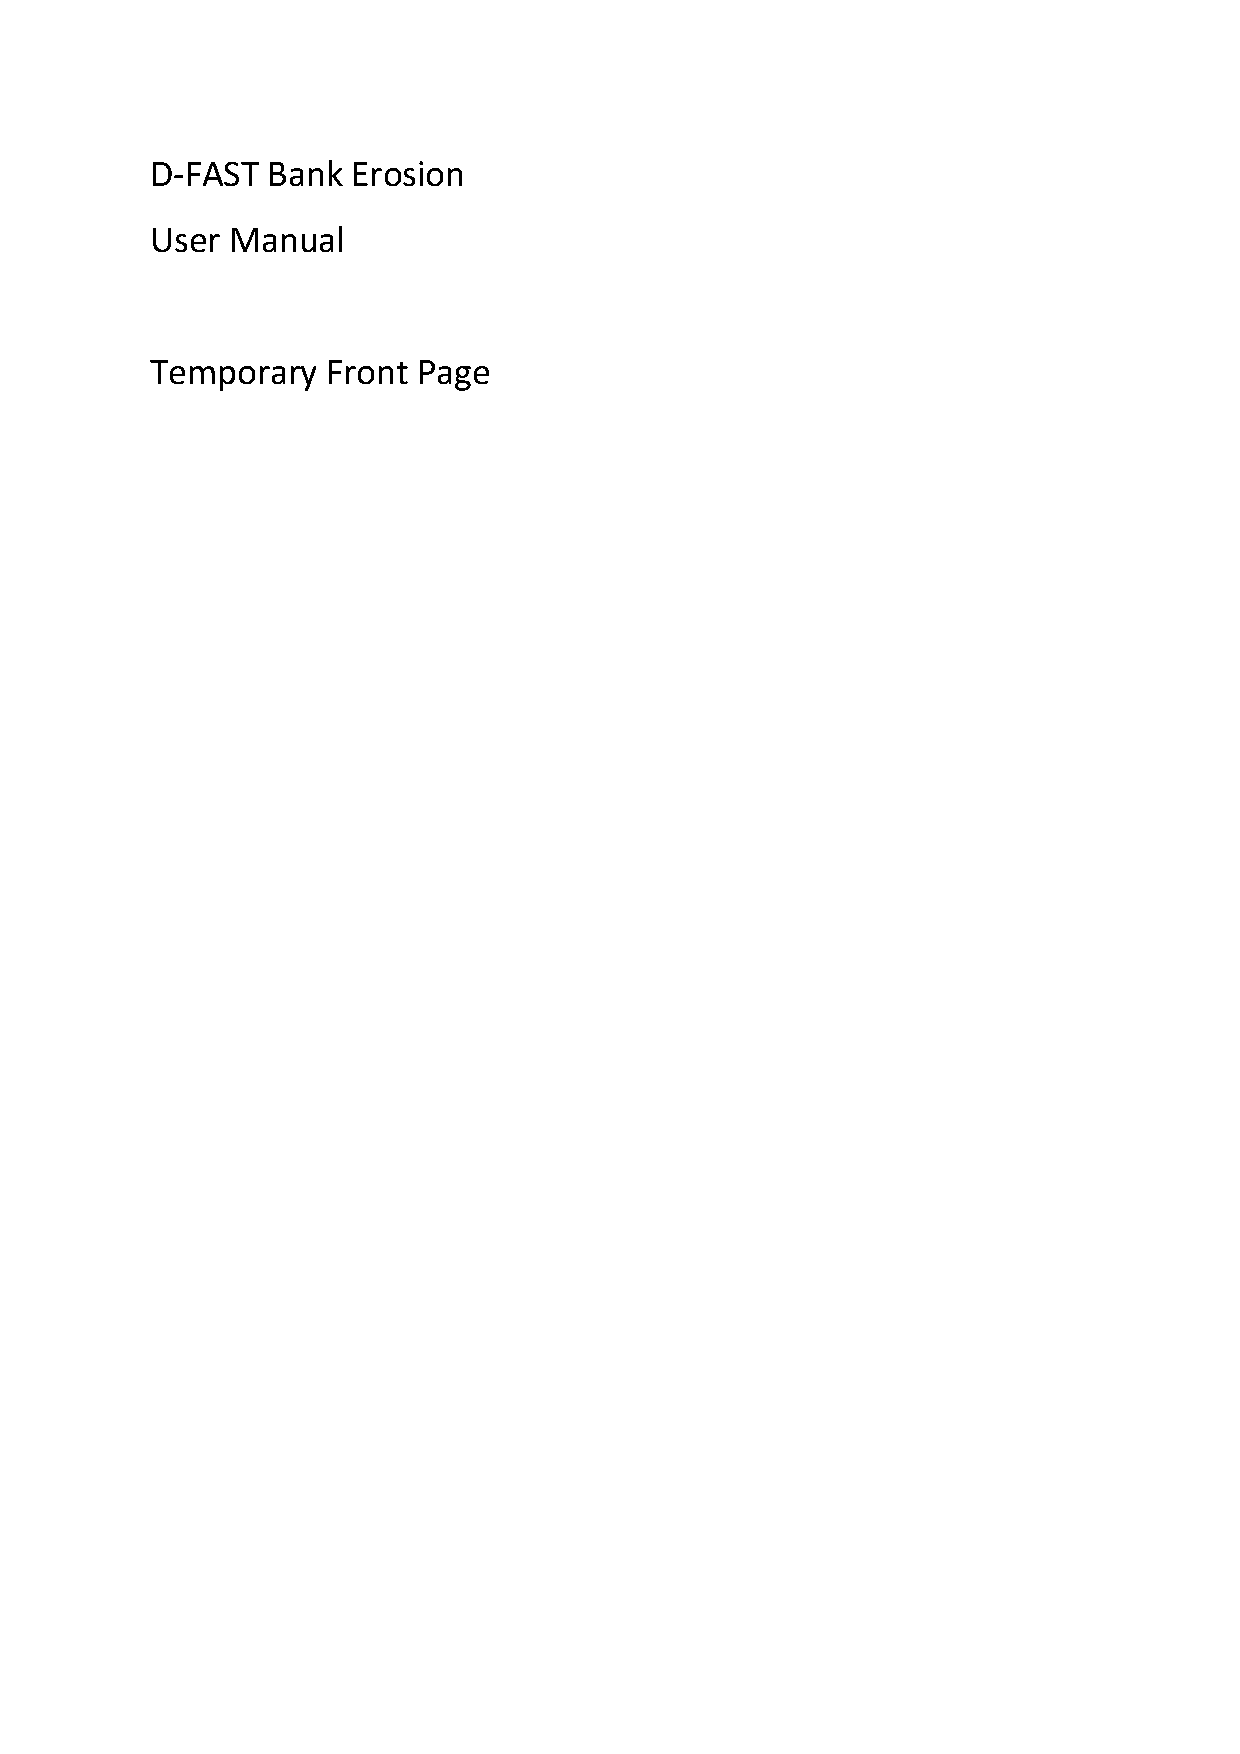
\includepdf[pages=1, offset=72 -70]{cover/d-fast-bank-erosion.pdf} % links-rechts past precies
%\cleardoublepage
\title{D-FAST\\ Bank Erosion}
\subtitle{}
\manualtype{Technical Reference Manual}
\version{1.0}

\author{Bert Jagers}

\deltarestitle
%
\chapter{Introduction}

This document describes the code design considerations for the development of \dfastbe.
\dfastbe is the successor of WAQBANK.
The purpose of these tools is to provide an estimate of the bank erosion due to currents and shipping.
The conceptual WAQBANK framework was developed since 2010.
To obtain the estimate of the bank erosion, the algorithm needs data on e.g.

\begin{itemize}
\item velocity distribution at a number of representative discharges,
\item bank composition and protection, and
\item shipping characteristics.
\end{itemize}

Based on these data the algorithm provides estimates of the average and maximum erosion distances along the studied reach after a characteristic period, and when the ultimate equilibrium conditions have been reached.
The original WAQBANK tool performs the analysis based on results obtained from WAQUA or Delft3D 4 simulations.
The new \dfastbe tool performs the analysis based on D-Flow FM simulation results.

\chapter{Software Requirements}

\section{Introduction}

The new program is to replace WAQBANK which was developed for the SIMONA system.
The essence of the requirements is that the new code should be consistent with the WAQBANK version except for the fact that it supports new \dflowfm map-files.

WAQBANK consists of two components:

\begin{enumerate}
\item the first component to determine the location of bank lines based on simulation results and a reference bank line (e.g.~from Baseline)
\item the second component to determine the bank erosion along that line based on simulation results and user input.
\end{enumerate}

The input of WAQBANK consists of one configuration using an ini-file like syntax which includes references to SIMONA or Delft3D 4 simulation files, and various simple ASCII files containing analysis parameters varying along the river reach.
The output of WAQBANK consists of a number of simple ASCII files reporting on the erosion volumes per reach segment (e.g.~per km) and a number of files listing the new coordinates of the bank lines after erosion.
Finally, the WAQBANK program may write some data in file formats suitable for visualization in WAQVIEW and generate a number of figures.

\section{Functional Requirements} \label{Sec:FuncReq}

\begin{enumerate}
\item The results of this program must match those of WAQBANK given the same input data.
\item Users must be able to run this program in batch mode from the command line.
\item Users must be able to run the analysis based on \dflowfm results.
\item Users must be able to provide all data via an input file, similar to the ini-file like file of WAQBANK.
\item The input files must be consistent with those of WAQBANK, or aligned with open standards or the \dflowfm modeling system.
\item The output files must be consistent with those of WAQBANK, or aligned with open standards or the \dflowfm modeling system.

\item The should read relevant data directly from \dflowfm map-files similarly to WAQBANK reading data directly from SIMONA and Delft3D 4 result files.

\item A simple graphical user interface could support users in process of creating the input file.

\item It would be nice if the software would be more generally applicable than just the Dutch rivers.
\item It would be nice if the software would be able to run besides English also in Dutch.
\end{enumerate}

\section{Non-functional requirements}

\begin{enumerate}
\item The performance of the tools must be similar to that of WAQBANK, i.e.~it must run within about an hour.
\item The software must be version controlled.
\item The software must have formal testing and support.
\item The software must run on Windows.
\item The software must be easy to distribute.
\item The software must have a user manual.
\item The software must have technical documentation.
\item The software must meet the conditions described in \href{http://publicaties.minienm.nl/documenten/rijkswaterstaat-informatievoorziening-aansluitvoorwaarden-riva-2017}{Rijkswaterstaat Informatievoorziening Aansluitvoorwaarden}.

\item The software should run on any common operating system.
\item The software should be available as open source.
\end{enumerate}
\chapter{Code structure}

\dfastbe code is subdivided into 7 files:

\begin{itemize}
	\item \file{\_\_init\_\_.py} module level file containing mainly the version number.
	\item \file{\_\_main\_\_.py} module level file containing argument parsing and call to \keyw{dfastbe.cmd.run()}.
	\item \file{base\_calculator.py} defining a parent \keyw{BaseCalculator} class for bank line detection and erosion steps.
	\item \file{cmd.py} containing the main run routine.
	\item \file{plotting.py} containing routines to visualize the results.
	\item \file{resources.py} is used to link to the \dfastbe logo.
	\item \file{utils.py} containing some utility functions.
\end{itemize}

and 4 sub-packages:

\begin{itemize}
	\item \file{bank\_lines} implements the workflow for the bank line detection analysis (triggered either by a \keyw{-{}-mode banklines} call or by clicking the \button{Detect} button in the graphical user interface).
	\item \file{bank\_erosion} implements the workflow for the bank line erosion analysis (triggered either by a \keyw{-{}-mode bankerosion} call or by clicking the \button{Compute} button in the graphical user interface).
	\item \file{gui} contains all functionality related to the graphical user interface.
	\item \file{io} contains the reading, parsing and writing of all configuration and result files.
\end{itemize}

The detailed description of the code per class and routine is beyond the scope of this document.
For more details the reader is referred to the documentation strings included in the source code.

\chapter{Software maintenance}

\section{Coding guidelines}

This program has been implemented following the Python PEP 8 style guide using Python 3.8.
The code has been documented using standard Python docstrings and type hinting.
For the static type checker \emph{mypy} is used.

\begin{Verbatim}
    > conda install mypy
    > mypy dfastbe
\end{Verbatim}

Variables associated with NumPy, netCDF4 and PyQt5 are not yet properly type checked.

\begin{Verbatim}[fontsize=\tiny]
> mypy dfastbe
dfastbe\plotting.py:31: error: Skipping analyzing 'shapely': found module but no type hints or library stubs
dfastbe\plotting.py:33: error: Skipping analyzing 'matplotlib': found module but no type hints or library stubs
dfastbe\plotting.py:34: error: Skipping analyzing 'matplotlib.pyplot': found module but no type hints or library stubs
dfastbe\plotting.py:35: error: Skipping analyzing 'geopandas': found module but no type hints or library stubs
dfastbe\plotting.py:36: error: Skipping analyzing 'numpy': found module but no type hints or library stubs
dfastbe\kernel.py:32: error: Skipping analyzing 'numpy': found module but no type hints or library stubs
dfastbe\io.py:32: error: Skipping analyzing 'numpy': found module but no type hints or library stubs
dfastbe\io.py:33: error: Skipping analyzing 'pandas': found module but no type hints or library stubs
dfastbe\io.py:34: error: Skipping analyzing 'geopandas': found module but no type hints or library stubs
dfastbe\io.py:35: error: Skipping analyzing 'shapely': found module but no type hints or library stubs
dfastbe\io.py:52: error: Skipping analyzing 'netCDF4': found module but no type hints or library stubs
dfastbe\support.py:36: error: Skipping analyzing 'numpy': found module but no type hints or library stubs
dfastbe\support.py:38: error: Skipping analyzing 'shapely': found module but no type hints or library stubs
dfastbe\support.py:39: error: Skipping analyzing 'geopandas': found module but no type hints or library stubs
dfastbe\batch.py:40: error: Skipping analyzing 'geopandas': found module but no type hints or library stubs
dfastbe\batch.py:41: error: Skipping analyzing 'shapely': found module but no type hints or library stubs
dfastbe\batch.py:43: error: Skipping analyzing 'numpy': found module but no type hints or library stubs
dfastbe\batch.py:44: error: Skipping analyzing 'matplotlib': found module but no type hints or library stubs
dfastbe\gui.py:32: error: Skipping analyzing 'PyQt5': found module but no type hints or library stubs
dfastbe\gui.py:34: error: Skipping analyzing 'PyQt5.QtGui': found module but no type hints or library stubs
dfastbe\gui.py:41: error: Skipping analyzing 'matplotlib.pyplot': found module but no type hints or library stubs
dfastbe\gui.py:41: error: Skipping analyzing 'matplotlib': found module but no type hints or library stubs
dfastbe\gui.py:1580: error: Cannot assign to a method
dfastbe\gui.py:1580: error: Incompatible types in assignment (expression has type "Type[str]", variable has type "Callable[[str], str]")
dfastbe\cmd.py:32: error: Skipping analyzing 'matplotlib.pyplot': found module but no type hints or library stubs
dfastbe\cmd.py:32: error: Skipping analyzing 'matplotlib': found module but no type hints or library stubs
dfastbe\cmd.py:36: error: Skipping analyzing 'numpy': found module but no type hints or library stubs
dfastbe\__main__.py:46: error: Skipping analyzing 'pyproj.datadir': found module but no type hints or library stubs
dfastbe\__main__.py:46: note: See https://mypy.readthedocs.io/en/latest/running_mypy.html#missing-imports
dfastbe\__main__.py:46: error: Skipping analyzing 'pyproj': found module but no type hints or library stubs
dfastbe\__main__.py:51: error: Skipping analyzing 'fiona.ogrext': found module but no type hints or library stubs
dfastbe\__main__.py:51: error: Skipping analyzing 'fiona': found module but no type hints or library stubs
dfastbe\__main__.py:52: error: Skipping analyzing 'fiona._shim': found module but no type hints or library stubs
dfastbe\__main__.py:53: error: Skipping analyzing 'fiona.schema': found module but no type hints or library stubs
dfastbe\__main__.py:54: error: Cannot find implementation or library stub for module named '_ctypes'
dfastbe\__main__.py:55: error: Skipping analyzing 'pandas._libs.tslibs.base': found module but no type hints or library stubs
dfastbe\__main__.py:55: error: Skipping analyzing 'pandas': found module but no type hints or library stubs
dfastbe\__main__.py:55: error: Skipping analyzing 'pandas._libs': found module but no type hints or library stubs
dfastbe\__main__.py:55: error: Skipping analyzing 'pandas._libs.tslibs': found module but no type hints or library stubs
dfastbe\__main__.py:58: error: Skipping analyzing 'netCDF4.utils': found module but no type hints or library stubs
dfastbe\__main__.py:58: error: Skipping analyzing 'netCDF4': found module but no type hints or library stubs
dfastbe\__main__.py:59: error: Skipping analyzing 'cftime': found module but no type hints or library stubs
dfastbe\__main__.py:60: error: Skipping analyzing 'matplotlib.backends.backend_qt5': found module but no type hints or library stubs
dfastbe\__main__.py:60: error: Skipping analyzing 'matplotlib': found module but no type hints or library stubs
dfastbe\__main__.py:60: error: Skipping analyzing 'matplotlib.backends': found module but no type hints or library stubs
Found 44 errors in 8 files (checked 9 source files)
\end{Verbatim}

The final two errors reported for \keyw{dfastbe\textbackslash{}gui.py} (line: 1451) are caused by a statement to switch the configparser to case sensitive mode while creating the data structure to be saved to file; most likely the data type is not properly set in the configparser definition.
That code line conforms to the configparser documentation and works properly as is.

A consistent coding style is enforced by means of the \emph{Black Code Formatter}.

\begin{Verbatim}
    > conda install black
    > black dfastbe
\end{Verbatim}

\section{Version control}

GitHub is currently used for software version control.
The repository is located at \url{https://github.com/Deltares/D-FAST_Bank_Erosion}.
Since \dfastbe builds on WAQBANK, the initial release of the new Python product is labeled as version 2.0.0.
%We may switch to GitLab in line with \href{http://publicaties.minienm.nl/documenten/rijkswaterstaat-informatievoorziening-aansluitvoorwaarden-riva-2017}{RIVA (2020)}.

\section{Automated building of code}

An automated TeamCity project will be set up for building and signing of binaries.
This is ongoing work; the build steps are currently run locally.
The Nuitka compiler is used to build a binary by means of the following command

\begin{Verbatim}
nuitka --standalone --python-flag=no_site --show-progress
    --plugin-enable=numpy --plugin-enable=qt-plugins
    --plugin-enable=tk-inter --file-reference-choice=runtime dfastbe
\end{Verbatim}

Unfortunately, this doesn't automatically build a binary that works out of the box.
The following adjustments depend on the exact combination of Nuitka and package versions used, so they will need to be revisited when updating the software.
A number of explicit module imports and environmental settings had to be added to \keyw{\_\_main\_\_} which the Nuitka compiler didn't automatically resolve.

\begin{Verbatim}
#------------------------------------------------------------------------------
# Needed for Nuitka compilation
#------------------------------------------------------------------------------
import os
import pathlib

is_nuitka = "__compiled__" in globals()
if is_nuitka:
    root = str(pathlib.Path(__file__).parent)
    os.environ["GDAL_DATA"] = root + os.sep + "gdal"
    os.environ["PROJ_LIB"] = root + os.sep + "proj"
    os.environ["MATPLOTLIBDATA"] = root + os.sep + "matplotlib" + os.sep + "mpl-data"
    os.environ["TCL_LIBRARY"] = root + os.sep + "lib" + os.sep + "tcl8.6"
    proj_lib_dirs = os.environ.get("PROJ_LIB", "")
    import pyproj.datadir
    pyproj.datadir.set_data_dir(root + os.sep + "proj")
    import pyproj

import fiona.ogrext
import fiona._shim
import fiona.schema
import _ctypes
import pandas._libs.tslibs.base
import pyproj._compat
import netCDF4.utils
import cftime
import matplotlib.backends.backend_qt5
#------------------------------------------------------------------------------
\end{Verbatim}

If these import statements are not included, you will sooner or later get a runtime error such as

\begin{Verbatim}
File "netCDF4\_netCDF4.pyx", line 1196, in init netCDF4._netCDF4
 ModuleNotFoundError: No module named 'netCDF4.utils'
\end{Verbatim}

Finally, the a number of directory creation and copy statements had to be executed to complete the build process where the Python environment was installed in \keyw{\%ENV\%}.
These statements are included in the \keyw{build\_dfastbe.bat} file.
The message "The code execution cannot proceed because python38.dll was not found. Reinstalling the program may fix this problem." is solved by executing

\begin{Verbatim}
copy %ENV%\python38.dll dfastbe.dist
\end{Verbatim}

The error "FileNotFoundError: [Errno 2] No such file or directory: '...\textbackslash{}dfastbe.dist\textbackslash{}certifi\textbackslash{}cacert.pem'" in the open\_binary routine within "importlib\textbackslash{}resources.py", line 97, is solved by

\begin{Verbatim}
mkdir dfastbe.dist\certifi
copy %ENV%\Lib\site-packages\certifi\cacert.pem dfastbe.dist\certifi
\end{Verbatim}

The error "pyproj.exceptions.DataDirError: Valid PROJ data directory not found. Either set the path using the environmental variable PROJ\_LIB or with `pyproj.datadir.set\_data\_dir`." in the get\_data\_dir function within "pyproj\textbackslash{}datadir.py", line 109, is solved by

\begin{Verbatim}
mkdir dfastbe.dist\proj
copy %ENV%\Lib\site-packages\pyproj\proj_dir\share\proj\* dfastbe.dist\proj
\end{Verbatim}

When the error "OSError: Could not find lib geos\_c.dll or load any of its variants []." is encountered in the load\_dll routine within "shapely\textbackslash{}geos.py", line 60, the following lines are needed

\begin{Verbatim}
mkdir dfastbe.dist\shapely\DLLs
copy %ENV%\Lib\site-packages\shapely\DLLs\* dfastbe.dist\shapely\DLLs
\end{Verbatim}

The message "StopIteration" in the file "geopandas\textbackslash{}datasets\textbackslash{}\_\_init\_\_.py", line 6, is caused by missing geopandas datasets and it is resolve by

\begin{Verbatim}
mkdir dfastbe.dist\geopandas\datasets
copy %ENV%\Lib\site-packages\geopandas\datasets\natural* dfastbe.dist\geopandas\datasets
\end{Verbatim}

%The error "ImportError: unable to find Qt5Core.dll on PATH" in the find\_qt routine within "PyQt5\textbackslash{}\_\_init\_\_.py", line 33, is resolved by
%
%\begin{Verbatim}
%mkdir dfastbe.dist\PyQt5\Qt\bin
%copy %ENV%\Library\bin\Qt5Core* dfastbe.dist\PyQt5\Qt\bin
%\end{Verbatim}

The import error "LoadLibraryExW 'fiona\textbackslash{}ogrext.pyd' failed: The specified module could not be found." in "fiona\textbackslash{}collection.py", line 9, whereas the ogrext.pyd is exactly where the program indicates, is caused by a large number of missing library dependencies (the boost libraries don't seem to be needed, so remove them after the copy)

\begin{Verbatim}
copy %ENV%\Library\bin\*.dll dfastbe.dist
del /y dfastbe.dist/boost*.dll
\end{Verbatim}

The import error "LoadLibraryExW '\_ctypes.pyd' failed: The specified module could not be found." is solved by adding one more library from another folder

\begin{Verbatim}
copy %ENV%\DLLs\libffi-7.dll dfastbe.dist
\end{Verbatim}

The runtime error "Could not find the matplotlib data files" in the \_get\_data\_path function within "matplotlib\textbackslash{}\_\_init\_\_.py", line 772, is solved by running

\begin{Verbatim}
del /s /y dfastbe.dist\mpl-data
mkdir dfastbe.dist\matplotlib\mpl-data
xcopy /s /y %ENV%\Lib\site-packages\matplotlib\mpl-data\* dfastbe.dist\matplotlib\mpl-data
\end{Verbatim}

Note that as the first action we delete the mpl-data folder created by Nuitka; it seems to be in the wrong place.
The operating system error "could not find or load spatialindex\_c-64.dll" in "rtree\textbackslash{}core.py", line 126, is solved by two libraries with similar names

\begin{Verbatim}
mkdir dfastbe.dist\Library\bin
copy %ENV%\Library\bin\spatialindex* dfastbe.dist\Library\bin
\end{Verbatim}

%The import error "LoadLibraryExW 'PyQt5\textbackslash{}QtWidgets.pyd' failed: The specified module could not be found." in "dfastbe\textbackslash{}gui.py", line 32, is caused by a large number of missing libraries for PyQt5
%
%\begin{Verbatim}
%copy %ENV%\python3.dll dfastbe.dist\PyQt5
%copy dfastbe.dist\*.dll dfastbe.dist\PyQt5
%\end{Verbatim}

The runtime error "Unable to load language file 'messages.UK.ini'." (and the lack of icons in the dialog) is simply solved by adding the configuration files to a new subdirectory dfastbe as

\begin{Verbatim}
mkdir dfastbe.dist\dfastbe
copy dfastbe\messages.*.ini dfastbe.dist\dfastbe
copy dfastbe\*.png dfastbe.dist\dfastbe
\end{Verbatim}

The message "qt.qpa.plugin: Could not find the Qt platform plugin 'windows' in ''. This application failed to start because no Qt platform plugin could be initialized. Reinstalling the application may fix this problem." is solved by adding the platforms folder to the distribution

\begin{Verbatim}
mkdir dfastbe.dist\platforms
xcopy /s /y %ENV%\Library\plugins\platforms\* dfastbe.dist\platforms
\end{Verbatim}

By default matplotlib uses Tk for graphics; to resolve some stability issues with the compiled code, we have changed to the Qt5 environment consistent with the rest of the user interface.
Unfortunatly, the overall code still depends on the Tcl/Tk environment.
The message "\_tkinter.TclError: Can't find a usable init.tcl in the following directories: <directory list> This probably means that Tcl wasn't installed properly." is solved by

\begin{Verbatim}
del /s /y dfastbe.dist\tcl
mkdir dfastbe.dist\lib\tcl8.6
xcopy /s /y %ENV%\Library\lib\tcl8.6\* dfasstbe.dist\lib\tcl8.6
\end{Verbatim}

where the first line removes the tcl folder created by Nuitka.
The related message "\_tkinter.TclError: Can't find a usable tk.tcl in the following directories: <directory list> rem This probably means that tk wasn't installed properly." in "tkinter\textbackslash{}\_\_init\_\_.py", line 2261, is solved by the similar lines (again removing the tk folder created by Nuitka)

\begin{Verbatim}
del /s /y dfastbe.dist\tk
mkdir dfastbe.dist\lib\tk8.6
xcopy /s /y %ENV%\Library\lib\tk8.6\* dfasstbe.dist\lib\tk8.6
\end{Verbatim}

The location where we need to copy the Tcl and Tk libraries depends on the environmental variable \keyw{TCL\_LIBRARY} set in the \keyw{\_\_main\_\_} routine.

\section{Listing of external modules}

The code has been developed in an Anaconda Python 3.8 environment including the following modules and versions.

\begin{Verbatim}
# Name                    Version                   Build  Channel
appdirs                   1.4.4                      py_0
atomicwrites              1.4.0                      py_0
attrs                     20.3.0             pyhd3eb1b0_0
black                     19.10b0                    py_0
blas                      1.0                         mkl
bzip2                     1.0.8                he774522_0
ca-certificates           2020.10.14                    0
certifi                   2020.12.5        py38haa95532_0
cfitsio                   3.470                he774522_6
cftime                    1.3.0            py38h347fdf6_0    conda-forge
click                     7.1.2                      py_0
click-plugins             1.1.1                      py_0
cligj                     0.7.1            py38haa95532_0
colorama                  0.4.4                      py_0
curl                      7.71.1               h4b64cdc_8    conda-forge
cycler                    0.10.0                     py_2    conda-forge
descartes                 1.1.0                      py_4    conda-forge
expat                     2.2.10               h33f27b4_2
fiona                     1.8.18           py38h60f4e94_0    conda-forge
freetype                  2.10.4               h546665d_0    conda-forge
freexl                    1.0.6                h2bbff1b_0
gdal                      3.1.4            py38h8f7194f_0    conda-forge
geopandas                 0.8.1                      py_0
geos                      3.8.1                he025d50_0    conda-forge
geotiff                   1.6.0                h8884d1a_3    conda-forge
gettext                   0.19.8.1          hb01d8f6_1002    conda-forge
glib                      2.65.0               he4de6d7_0    conda-forge
hdf4                      4.2.13               h712560f_2
hdf5                      1.10.6          nompi_h5268f04_1112    conda-forge
icc_rt                    2019.0.0             h0cc432a_1
icu                       67.1                 h33f27b4_0    conda-forge
iniconfig                 1.1.1                      py_0
intel-openmp              2020.2                      254
jpeg                      9d                   h8ffe710_0    conda-forge
kealib                    1.4.14               ha3510f1_0    conda-forge
kiwisolver                1.3.1            py38hbd9d945_0    conda-forge
krb5                      1.17.2               hbae68bd_0    conda-forge
libboost                  1.67.0               hd9e427e_4
libclang                  10.0.1          default_hf44288c_1    conda-forge
libcurl                   7.71.1               h4b64cdc_8    conda-forge
libffi                    3.2.1             ha925a31_1007    conda-forge
libgdal                   3.1.4                h0e5aa5a_0    conda-forge
libiconv                  1.15                 h1df5818_7
libkml                    1.3.0                he5f2a48_4
libnetcdf                 4.7.4           nompi_h2ee746f_106    conda-forge
libpng                    1.6.37               h2a8f88b_0
libpq                     12.3                 hd9aa61d_2    conda-forge
libspatialindex           1.9.3                h33f27b4_0
libspatialite             5.0.0                hf693123_0    conda-forge
libssh2                   1.9.0                h7a1dbc1_1
libtiff                   4.1.0                hc10be44_6    conda-forge
libwebp-base              1.1.0                h8ffe710_3    conda-forge
libxml2                   2.9.10               hb89e7f3_3
lz4-c                     1.9.2                h62dcd97_2    conda-forge
m2w64-expat               2.1.1                         2
m2w64-gcc-libgfortran     5.3.0                         6
m2w64-gcc-libs            5.3.0                         7
m2w64-gcc-libs-core       5.3.0                         7
m2w64-gettext             0.19.7                        2
m2w64-gmp                 6.1.0                         2
m2w64-libiconv            1.14                          6
m2w64-libwinpthread-git   5.0.0.4634.697f757               2
m2w64-xz                  5.2.2                         2
matplotlib                3.3.3            py38haa244fe_0    conda-forge
matplotlib-base           3.3.3            py38h34ddff4_0    conda-forge
mkl                       2020.2                      256
mkl-service               2.3.0            py38h196d8e1_0
mkl_fft                   1.2.0            py38h45dec08_0
mkl_random                1.1.1            py38h47e9c7a_0
more-itertools            8.6.0              pyhd3eb1b0_0
msys2-conda-epoch         20160418                      1
munch                     2.5.0                      py_0
mypy                      0.790                      py_0
mypy_extensions           0.4.3                    py38_0
netcdf4                   1.5.5           nompi_py38h5338a22_100    conda-forge
nuitka                    0.6.10             pyhd3eb1b0_0
numpy                     1.19.2           py38hadc3359_0
numpy-base                1.19.2           py38ha3acd2a_0
olefile                   0.46               pyh9f0ad1d_1    conda-forge
openjpeg                  2.3.1                h48faf41_3    conda-forge
openssl                   1.1.1h               he774522_0
packaging                 20.7               pyhd3eb1b0_0
pandas                    1.1.3            py38ha925a31_0
pathspec                  0.7.0                      py_0
pcre                      8.44                 ha925a31_0
pillow                    8.0.1            py38hd8d9125_0    conda-forge
pip                       20.3.1           py38haa95532_0
pluggy                    0.13.1                   py38_0
poppler                   0.89.0               h0cd1227_0    conda-forge
poppler-data              0.4.10                        0    conda-forge
postgresql                12.3                 he14cc48_2    conda-forge
proj                      7.1.1                h7d85306_3    conda-forge
psutil                    5.7.2            py38he774522_0
py                        1.9.0                      py_0
pyparsing                 2.4.7              pyh9f0ad1d_0    conda-forge
pyproj                    2.6.1.post1      py38hbdc76b6_3    conda-forge
pyqt                      5.12.3           py38h7ae7562_4    conda-forge
pyqt5-sip                 4.19.18                  pypi_0    pypi
pyqtchart                 5.12                     pypi_0    pypi
pyqtwebengine             5.12.1                   pypi_0    pypi
pytest                    6.1.2            py38haa95532_0
python                    3.8.5                h5fd99cc_1
python-dateutil           2.8.1                      py_0
python_abi                3.8                      1_cp38    conda-forge
pytz                      2020.4             pyhd3eb1b0_0
qt                        5.12.9               hb2cf2c5_0    conda-forge
regex                     2020.11.13       py38h2bbff1b_0
rtree                     0.9.4            py38h21ff451_1
setuptools                51.0.0           py38haa95532_2
shapely                   1.7.1            py38hc96c142_1    conda-forge
six                       1.15.0           py38haa95532_0
sqlite                    3.33.0               h2a8f88b_0
tbb                       2018.0.5             he980bc4_0
tiledb                    2.1.3                h968eb34_0    conda-forge
tk                        8.6.10               he774522_0
toml                      0.10.1                     py_0
tornado                   6.1              py38h294d835_0    conda-forge
typed-ast                 1.4.1            py38he774522_0
typing_extensions         3.7.4.3                    py_0
vc                        14.2                 h21ff451_1
vs2015_runtime            14.27.29016          h5e58377_2
wheel                     0.36.1             pyhd3eb1b0_0
wincertstore              0.2                      py38_0
xerces-c                  3.2.3                ha925a31_0
xz                        5.2.5                h62dcd97_0
zlib                      1.2.11               h62dcd97_4
zstd                      1.4.5                h1f3a1b7_2    conda-forge
\end{Verbatim}

\section{Automated testing of code}

See \autoref{Chp:TestPlan} and \autoref{Chp:TestReport}.

\section{Automated generation of documentation}

The documentation has been written in a combination of LaTeX and markdown files which are maintained in the GitHub repository alongside the source code.
The PDF version of the user manual and this technical reference manual are generated automatically as part of the daily cycle of building all manuals on the Deltares TeamCity server.
\chapter{Test Plan} \label{Chp:TestPlan}

The results of the software is verified by means of

\begin{itemize}
\item Unit testing at the level of functions, such as reading and writing of files, and basic testing of the algorithms.
Currently about half of the functions included in \keyw{io.py} are covered by unit tests; more to be added.
These tests are carried out by means of the \keyw{pytest} framework.
\item Regression tests have to configured to verify that the results of the batch mode remain unchanged under further code developments.
\end{itemize}

For the verification of \dfastbe three sets of input files for the Meuse River have been used:

\begin{enumerate}
\item One set of WAQUA result files converted using \keyw{sim2ugrid.m} to \dflowfm like netCDF files.
\item One set of \dflowfm result files of simulations using the same curvilinear mesh as was used in WAQUA.
\item One set of \dflowfm result files of simulations using a new unstructured mesh.
\end{enumerate}

Each configuration gives slightly different results; for further regression testing in particular the first and last one will be used.
For the automated testing, unit tests and regression tests based on known input/output combinations will be used.
These tests will be executed on the original Python code (i.e. in source code form) and to the degree possible on the compiled binaries as well.

\section{Acceptance testing}

In \autoref{Sec:FuncReq} the 10 functional requirements were listed.
They are repeated below and for every requirement it is indicated how it is tested.

\begin{enumerate}
\item The results of \dfastbe must match those of WAQBANK given the same input data.
This is tested by means of a number of comparison studies, and subsequently tested using regression tests.

\item Users must be able to run this program in batch mode from the command line.
This has been implemented as run modes \keyw{--mode banklines} and \keyw{--mode bankerosion}.
The proper functioning of these options is tested by means of regression testing.

\item Users must be able to run the analysis based on \dflowfm results.
This is tested by means of regression testing using result files of \dflowfm version X.

\item Users must be able to provide all data via an input file, similar to the ini-file like file of WAQBANK.
This testing is included in the regression testing of the batch mode, and may in the future be included in the gui testing.

\item The input files must be consistent with those of WAQBANK, or aligned with open standards or the \dflowfm modeling system.
The \dfastbe configuration file is identical to the WAQBANK definition file except for the fact that the new file contains three sections \keyw{[General]}, \keyw{[Detect]} and \keyw{[Erosion]} to give a bit more context for the purpose of each keyword.
\dfastbe accepts old WAQBANK input files, but writes the data in the new format.
The format of the other input files is not adjusted, but for line geometries \dfastbe also accepts shape files besides the original \file{.xyc} files.
There are unit and integration tests addressing the reading of the input files.

\item The output files must be consistent with those of WAQBANK, or aligned with open standards or the \dflowfm modeling system.
The ASCII files containing the bank erosion volumes are identical to those of WAQBANK.
The shifted bank lines are exported as Shape files instead of \file{.xyc} files to align with common GIS standards.
The figures are now saved as \file{.png} files instead of MATLAB specific \file{.fig} files.
There are unit and integration tests addressing the writing of the output files.

\item The should read relevant data directly from \dflowfm map-files similarly to WAQBANK reading data directly from SIMONA and Delft3D 4 result files.
All quantities previously read from the SIMONA SDS-files and Delft3D-FLOW trim-files is now read from the \dflowfm map.nc files.

\item A simple graphical user interface could support users in process of creating the input file.
The graphical user interface that you get by running \dfastbe in default mode or by explicitly specifying \keyw{--mode gui} has been tested manually as described in \autoref{Sec:GuiTests}.

\item It would be nice if the software would be more generally applicable than just the Dutch rivers.
The code does not include specific knowledge of the Dutch rivers except for the fact that some of the rules of thumb have been derived using Dutch river data.
The original WAQBANK code was already applied to foreign rivers such as the Danube.
No special testing carried out for this requirement.

\item It would be nice if the software would be able to run besides English also in Dutch.
All texts shown by \dfastbe are read from a language configuration file.
An English and a Dutch version of that configuration file are provided.
A most system tests are carried out using the default English configuration, but one test is carried out using the Dutch configuration.
\end{enumerate}

\section{System testing}

The whole system is tested via the command line (entry via \keyw{\_\_main\_\_}) and via Python calls to the \keyw{run} function in the \keyw{cmd} module.
These tests are repeated for the standalone compiled \dfastbe executable.
For the system testing a limited number of regression tests are carried out comparing the latest results against previously accepted results.

Since the testing of the graphical user interface is not included in the automated testing, a test protocol for manual tests has been defined.
These tests are described in the following section.

\subsection{Manual testing of the user interface} \label{Sec:GuiTests}

\subsubsection{Test 1: starting blank}
\subsubsection{Test 2: save default configuration file}
\subsubsection{Test 3: modify general settings}
\subsubsection{Test 4: modify detection settings}
\subsubsection{Test 5: modify erosion settings}
\subsubsection{Test 6: save modified configuration file}
\subsubsection{Test 7: load default configuration file}
\subsubsection{Test 8: load modified configuration file}
\subsubsection{Test 9: run detection analysis}
\subsubsection{Test 10: run erosion analysis}
\subsubsection{Test 11: view manual and about Windows}

\section{Integration testing}

The \keyw{batch} module builds on the functionality of the \keyw{io}, \keyw{support}, \keyw{kernel} and \keyw{plotting} modules to provide the bank line detection and erosion analysis functionality as main routines.
The main routines \keyw{banklines} and \keyw{bankerosion} are tested at this level via regression tests, the other routines in \keyw{batch} are tested as part of the unit testing.

\section{Unit testing}

Since the modules \keyw{io}, \keyw{support}, \keyw{kernel} and \keyw{plotting} only depend on third party modules, they are ideally suited for unit testing.
Most of the routines in \keyw{batch} can be addressed by means of unit testing as well.
An initial number of unit tests have been set up for \keyw{io} routines, more unit tests should be added.

All routines inside \keyw{gui} are interacting with the graphical user interface (either by extracting data from the state of the controls, or by setting the state of the controls).
These routines cannot be tested using the pytest framework, and are therefore tested by means of the manual system tests.

\section{Automated testing}

Automated TeamCity projects will be set up for testing the Python code, for building (and optionally signing of) binaries, and testing of the binaries.
In this way the formal release process can be easily aligned with the other products.
This is ongoing work; the test and build steps are currently run locally.

For all automated unit and regression tests the pytest framework is used.

\begin{Verbatim}
    > conda install pytest
    > pytest
\end{Verbatim}

%-------------------------------
\chapter{Test Report} \label{Chp:TestReport}

The test plan describes manual tests (the graphical user interface tests as part of the system testing) and automated testing (unit and regression testing).

\section{Manual tests}

This section summarizes the results of the manual testing of the graphical user interface.

\begin{tabular}{ll|l}
Test & Description & Success / Comments \\ \hline
1 & starting blank & OK \\
2 & save default configuration file & OK \\
3 & modify general settings & OK \\
4 & modify detection settings & OK \\
5 & modify erosion settings & OK \\
6 & save modified configuration file & OK \\
7 & load default configuration file & OK \\
8 & load modified configuration file & OK \\
9 & run detection analysis & OK \\
10 & run erosion analysis & OK \\
11 & view manual and about Windows & OK \\
\end{tabular}

\section{Automated tests}

Below a brief pytest report of the automated regression and unit testing is included.
Each period following a module name represents one successful test; failed test would be indicated by an F and a subsequent error report.

\begin{Verbatim}[fontsize=\tiny]
=============================================== test session starts ================================================
platform win32 -- Python 3.8.5, pytest-6.1.2, py-1.9.0, pluggy-0.13.1
rootdir: D:\checkouts\D-FAST\D-FAST_Bank_Erosion
collected 33 items

tests\test_io.py .................................                                                            [100%]

=============================================== 33 passed in 11.79s ================================================
\end{Verbatim}

%\markdownInput{techref.md}

%\nonumchapter{References}
%\bibliography{dfastbe}

\appendix
\chapter{File formats} \label{Chp:FileFormats}

The software distinguishes 9 files:

\begin{itemize}
\item The \emph{analysis configuration file} defines the settings that are relevant for the execution of the software, it will point to other data files for bulk data.
\item The \emph{line geometry files} specify the coordinates of a line.
\item The \emph{chainage file} defines the river chainage along a line.
\item The \emph{parameter files} define optional spatial variations in the analysis input parameters.
\item The \emph{simulation result files} define the spatial variations in the velocities and water depths as needed by the algorithm.
\item The \emph{eroded volume file} reports on the eroded volumes along the analyzed river reach per chainage bin.
\item The \emph{dialog text file} defines all strings to be used in the interaction with the users (GUI, report, or error messages).
\item The \emph{shape file} specify the detected and shifted bank lines; this format is also used for various debug output.
\item The \emph{image file} stores the figures created by the software; by default the PNG format is used.
\end{itemize}

Each file type is addressed separately in the following subsections.
The shape and image files follow commonly used formats and are hence not explained.

\section{analysis configuration file} \label{Sec:cfg}

The analysis configuration file of WAQBANK looked a lot like an ini-file, but deviated slightly due to different comment style and missing chapter blocks.
\dfastbe still supports the old files, but it's recommended to upgrade them to the newer file format described here which conforms to the usual ini-file format.
The user interface reads old (and obviously new) files, but always writes new files.

The file must contain a \keyw{[General]} block with a keyword \keyw{Version} to indicate the version number of the file.
The initial version number will be \keyw{1.0}.

Details on the other keywords supported are given below.
The order of the keywords in the file doesn't matter, but each block and each keyword should occur only once.

\begin{longtable}{l|l|p{8cm}}
%\begin{tabular}{l|l|p{8cm}}
Block & Keyword & Description \\ \hline
\keyw{General} & \keyw{Version} & Version number. Must be \keyw{1.0} \\
& \keyw{RiverKM} & Name of file with river chainage (kilometres) and corresponding xy-coordinates \\
& \keyw{Boundaries} & River chainage of the region of interest specified as rkm-start:rkm-end, e.g. 81:100 (default: all) \\
& \keyw{BankDir} & Directory for storing bank lines (default: current directory) \\
& \keyw{BankFile} & Name of file(s) in which xy-coordinates of bank lines are stored (default 'bankfile') \\
& \keyw{Plotting} & Flag indicating whether figures should be created (default: true) \\
& \keyw{SavePlots} & Flag indicating whether figures should be saved (default: true) \\
& \keyw{SaveZoomPlots} & Flag indicating whether additional figures should be saved containing zoomed in versions of the standard plots per specified chainage step (default: false) \\
& \keyw{ZoomStepKM} & Chainage step size for the zoom plots (default: 1) \unitbrackets{km} \\
& \keyw{ClosePlots} & Flag indicating whether figures should be closed when the run ends (default: false) \\
& \keyw{FigureDir} & Directory for storing figures (default relative to work dir: figure) \\
& \keyw{FigureExt} & String indicating the file extension and type to be used for the figures saved (default: .png) \\
& \keyw{DebugOutput} & Flag indicating whether additional debug output should be written; this includes various shape and csv files with intermediate results (default: false) \\

\keyw{Detect} & \keyw{SimFile} & Name of simulation output file to be used for determining representative bank line \\
& \keyw{WaterDepth} & Water depth used for defining bank line (default: 0.0) \\
& \keyw{NBank} & Number of bank lines, (default: 2) \\
& \keyw{Line<$i$>} & Name of file with xy-coordinates of search line \keyw{<$i$>} \\
& \keyw{DLines} & Distance from pre-defined lines used for determining bank lines (default: 50) \\

\keyw{Erosion} & \keyw{TErosion} & Simulation period \unitbrackets{years} \\
& \keyw{RiverAxis} & Name of file with xy-coordinates of river axis \\
& \keyw{Fairway} & Name of file with xy-coordinates of fairway axis \\
& \keyw{OutputInterval} & Bin size for which the eroded volume output is given (default: 1) \unitbrackets{km} \\
& \keyw{NLevel} & Number of discharge levels \\
& \keyw{RefLevel} & Reference level: discharge level with \keyw{SimFile<$i$>} that is equal to \keyw{SimFile} (only used when \keyw{Nlevel} > 1)  (default: 1) \\
& \keyw{SimFile<$i$>} & NetCDF map-file for computing bank erosion for discharge \keyw{<$i$>} (only used when \keyw{Nlevel} > 1) \\
& \keyw{PDischarge<$i$>} & Probability of discharge \keyw{<$i$>} (sum of probabilities should be 1) \\
& \keyw{OutputDir} & Directory for storing output files \\
& \keyw{BankNew} & Name of file(s) in which new xy-coordinates of bank lines are stored (default 'banknew') \\
& \keyw{BankEq} & Name of file(s) in which xy-coordinates of equilibrium bank lines are stored (default: 'bankeq') \\
& \keyw{EroVol} & Name of file in which eroded volume per river-km is stored (default: 'erovol.evo') \\
& \keyw{ShipType} & Constant or name of file containing type of ship (per river-km) \\
& \keyw{Vship} & Constant or name of file containing relative velocity of the ships (per river-km) \unitbrackets{m/s} \\
& \keyw{Nship} & Constant or name of file containing number of ships per year (per river-km) \\
& \keyw{Nwave} & Constant or name of file containing number of waves per ship (default 5) \\
& \keyw{Draught} & Constant or name of file containing draught of the ships (per river-km) \unitbrackets{m} \\
& \keyw{Wave0} & Constant or name of file containing distance from fairway axis at which wave height is zero (default 200) \unitbrackets{m} \\
& \keyw{Wave1} & Constant or name of file containing distance from fairway axis at which reduction of wave height to zero starts (default \keyw{Wave0} minus 50) \unitbrackets{m} \\
& \keyw{Classes} & Use classes (true) or critical shear stress (false) in \keyw{BankType} (default: true) \\
& \keyw{BankType} & Constant or \keyw{base} reference to files with bank strength definition (for each bank line per river-km) \\
& \keyw{ProtectionLevel} & Constant or \keyw{base} reference to files with level of bank protection for each bank line per river-km (default: -1000) \\
& \keyw{Slope} & Constant or \keyw{base} reference to files with equilibrium slope for each bank line per river-km  (default: 20) \\
& \keyw{Reed} & Constant or \keyw{base} reference to files with reed wave damping coefficient for each bank line per river-km  (default: 0) \\
& \keyw{VelFilterDist} & Specifies the distance/width of a moving average filter for the near bank velocities \unitbrackets{km} (default 0, meaning no filter applied) \\
& \keyw{BedFilterDist} & Specifies the distance/width of a moving average filter for the bank levels \unitbrackets{km} (default 0, meaning no filter applied)
%\end{tabular}
\end{longtable}

\Note When specifying chainage dependent values for \keyw{Slope}, \keyw{Reed}, \keyw{BankType} and \keyw{ProtectionLevel}, please follow the file name conventions listed in \autoref{Sec:parfile}.

\subsubsection*{Example}

\begin{Verbatim}
[General]
  Version         = 1.0
  RiverKM         = inputfiles\rivkm_20m.xyc
  Boundaries      = 68:230
  BankDir         = files\outputbanklines
  BankFile        = bankline

[Detect]
  SimFile         = inputfiles\SDS-krw3_00-q0075_map.nc
  WaterDepth      = 0.0
  NBank           = 2
  Line1           = inputfiles\oeverlijn_links_mod.xyc
  Line2           = inputfiles\oeverlijn_rechts_mod.xyc
  DLines          = [20,20]

[Erosion]
  TErosion        = 1
  RiverAxis       = inputfiles\maas_rivieras_mod.xyc
  Fairway         = inputfiles\maas_rivieras_mod.xyc
  NLevel          = 2
  RefLevel        = 1
  SimFile1        = inputfiles\SDS-krw3_00-q0075_map.nc
  PDischarge1     = 0.25
  SimFile2        = inputfiles\SDS-krw3_00-q1500_map.nc
  PDischarge2     = 0.75
  OutputDir       = files\outputbankerosion
  BankNew         = banknew
  BankEq          = bankeq
  EroVol          = erovol_standard.evo
  OutputInterval  = 0.1
  ShipType        = 2
  Vship           = 5.0
  Nship           = inputfiles\nships_totaal
  Nwave           = 5
  Draught         = 1.2
  Wave0           = 150.0
  Wave1           = 110.0
  Classes         = false
  BankType        = inputfiles\bankstrength_tauc
  ProtectionLevel = inputfiles\stortsteen
\end{Verbatim}

\section{line geometry files}

This file specifies the coordinates of a single line.
It is used to specify

\begin{itemize}
\item RiverAxis
\item Fairway
\item Initial bank (search) lines
\end{itemize}

The file format is equal to the file format used by WAQBANK.
It consists of two data columns: the first column specifies the x-coordinate and the second column the y-coordinate of each node of the line.

\subsubsection*{Example}

\begin{Verbatim}
1.1887425781300000e+005  4.1442128125000000e+005
1.1888840213863159e+005  4.1442400328947371e+005
1.1890254646426316e+005  4.1442672532894736e+005
1.1891669078989474e+005  4.1442944736842107e+005
1.1893083511552632e+005  4.1443216940789472e+005
1.1894497944115789e+005  4.1443489144736843e+005
1.1895912376678947e+005  4.1443761348684208e+005
1.1897326809242106e+005  4.1444033552631579e+005
1.1898741241805263e+005  4.1444305756578950e+005

...continued...
\end{Verbatim}

Shape files are used for all geospatial output, such as the detected bank lines and the shifted bank lines.

\section{chainage file}

This file defines the river chainage along a line.
The file format is equal to the file format used by WAQBANK.
It consists of three data columns: the first column specifies the chainage, the second and third columns specify the x- and y-coordinates of each node of the line.

\subsubsection*{Example}

\begin{Verbatim}
3     175908.078100      308044.062500
6     176913.890600      310727.781300
10     176886.578100     314661.750000
15     176927.328100     319589.687500
16     176357.000000     320335.375000 

...continued...
\end{Verbatim}

\section{parameter files} \label{Sec:parfile}

These files may be used to define spatial variations in the input parameters needed by the analysis.
Many parameters may be varied along the analyzed river reach.

\begin{itemize}
\item \keyw{wave0}: $s_0$ distance from ship at which the ship waves have reduced to zero \unitbrackets{m}
\item \keyw{wave1}: $s_1$ distance from ship at which the ship waves start to reduce \unitbrackets{m}
\item \keyw{vship}: $v_s$ ship sailing speed \unitbrackets{m/s}
\item \keyw{nship}: $N$ number of empty ships per year \unitbrackets{1/year}
\item \keyw{nwave}: $n$ number of waves per ship \unitbrackets{-}
\item \keyw{draught}: $T_s$ draught of the ship \unitbrackets{m}
\item \keyw{shiptype}: ship type \unitbrackets{-}
\item \keyw{slope}: $\mu_\text{fs}$ wave damping due to sloping foreshore \unitbrackets{m\textsuperscript{-1}} per bank, file extension \keyw{.slp}
\item \keyw{reed}: $\mu_r$ wave damping due to reed \unitbrackets{m\textsuperscript{-1}} per bank, file extension \keyw{.rdd}
\item \keyw{banktype}: bank type \unitbrackets{-} per bank, file extension \keyw{.btp}
\item \keyw{protectionlevel}: top level of the bank protection \unitbrackets{m} per bank, file extension \keyw{.bpl}
\end{itemize}

The file format is independent of the parameter for which it's used.
The file format is equal to the file format used by WAQBANK.
It consists of two data columns: the first column specifies the chainage and the second column the value at that location.
The chainage values should be increasing.
The values are used from the chainage specified on that line until the chainage specified on the next line.
The first value is also used before the chainage specified on the first line.
The last value is used for all chainages larger than the chainage specified on the last line.

\Note Some quantities (\keyw{Slope}, \keyw{Reed}, \keyw{BankType} and \keyw{ProtectionLevel}) need to be specified per bank.
For these parameters the user has to specify a number of files equal to the number of bank lines; for all other parameters only one file is expected that is used for all banks.
The names of the bank dependent files should equal \keyw{base\_1.ext}, \keyw{base\_2.ext}, {\it et cetera} where the user is free to choose \keyw{base} but the extension \keyw{.ext} depends on the quantity selected (see the list above).
The file extension and number part \keyw{\_i} should \emph{not} be included when specifying the file name in the analysis configuration file (see \autoref{Sec:cfg}) or associated user interface field.

\subsubsection*{Example}

\begin{Verbatim}
65.3    20912
67.6    18529
100.7   20375
146.8   24758
175.5   13911
201     15613
\end{Verbatim}

\section{simulation result files}

For the bank line detection and bank erosion analysis, the program  needs results from a hydrodynamic model.
The WAQBANK program was able to read data from the WAQUA SDS-output files or the Delft3D-FLOW trim-files.
\dfastbe now supports the results of \dflowfm in netCDF map-files following UGRID conventions.
The model needs the following data fields:

\begin{itemize}
\item x-coordinates of the mesh nodes
\item y-coordinates of the mesh nodes
\item face\_node\_connectivity of the mesh
\item bed levels zb at the mesh nodes
\item water levels zw at the mesh faces
\item water depths h at the mesh faces
\item velocity vector (ucx,ucy) at the mesh faces
\end{itemize}

The simulation result files may contain multiple time steps; the final time steps will be used for the analysis.


\section{eroded volume file}

This file reports on the eroded volumes per bank along the analyzed river reach per user defined chainage bin.
The file consists $1+N$ tab-separated data columns where $N$ is the number of bank lines processed: the first column specifies the chainage and the other columns report on the eroded bank volume per bank line accumulated be chainage bin.
The chainage coordinate provided is the upper limit of the chainage bin for which the volume is reported on that line.
The file format differs slightly from the file format used by WAQBANK since that file contained $N$ identical chainage columns followed by the $N$ eroded volume columns.

\subsubsection*{Example}

\begin{Verbatim}
68.00   2.21    0.00
68.10   6.44    0.00
68.20   7.81    0.00
68.30   43.63   161.39
68.40   14.24   0.00
68.50   8.88    0.00
68.60   0.00    0.00
68.70   0.00    0.00
68.80   2.39    0.00
68.90   0.00    0.00
69.00   0.88    0.00
69.10   7.40    69.27
69.20   5.64    65.47
69.30   11.98   55.78

...continued...
\end{Verbatim}

\section{dialog text file}

The dialog text file uses the block labels enclosed by square brackets of the common ini-file format, but the lines in between the blocks are treated verbatim and don't list keyword/value pairs.
Every print statement in the program is associated with a short descriptive identifier.
These identifiers show up in the dialog text file as the block labels.
The text that follows the block label will be used at that location in the program.
The order of the blocks in the file is not important.
Please note that every line is used as is, so don't add indentations or blank lines unless you want those to show up during the program execution.
Most blocks may contain any number of lines, but some blocks may only contain a single line.
Some data blocks may contain one or more Python-style placeholders used for inserting values.

\subsubsection*{Example}

The following excerpt of the default \keyw{messages.UK.cfg} dialog text file shows the string definition for 3 identifiers, namely \keyw{''} (the identifier for an empty line), \keyw{'header\_banklines'} and \keyw{'end\_banklines'}.
The header string contains two placeholders, namely \keyw{\{version\}} for the the version number and \keyw{\{location\}} for the url to the source code location.

\begin{Verbatim}
[]

[header_banklines]
=====================================================
Determine bank lines
=====================================================
version: {version}
source: {location}
-----------------------------------------------------
[end_banklines]

=====================================================
===        BankLines ended successfully!          ===
=====================================================
... continued ...
\end{Verbatim}

%\pagestyle{empty}
%\cleardoublepage
%\mbox{}
%\includepdf[pages=2, offset=-72 -70]{cover/d-fast-bank-erosion.pdf} % links-rechts past precies
\end{document}
